\documentclass[11pt]{article}
\usepackage[title]{appendix}
\usepackage[T1]{fontenc}
\usepackage[utf8]{inputenc}
\usepackage{lmodern}
\input{glyphtounicode}
\pdfgentounicode=1
\usepackage{amsmath,amssymb,amsthm,geometry,booktabs,tikz,hyperref}
\geometry{margin=1in}
\emergencystretch=1em
\hypersetup{colorlinks=true,linkcolor=blue,citecolor=blue,urlcolor=blue,pdftitle={A generalized pseudostandard prefix with no string attractor of size four},pdfauthor={P. Graham},pdfsubject={String attractors of pseudopalindromic prefixes of binary generalized pseudostandard sequences},pdfkeywords={string attractor, generalized pseudostandard sequence, palindromic closure, antipalindromic closure, combinatorics on words}}
\newtheorem{theorem}{Theorem}
\newtheorem{lemma}[theorem]{Lemma}
\newtheorem{proposition}[theorem]{Proposition}
\newtheorem{conjecture}[theorem]{Conjecture}
\theoremstyle{remark}
\newtheorem{remark}[theorem]{Remark}
\newcommand{\w}[1]{\textup{\texttt{#1}}}
\newcommand{\file}[1]{\texttt{\detokenize{#1}}}
\title{A generalized pseudostandard prefix with no string attractor of size four}
\author{P. Graham\\ \small\url{https://orcid.org/0009-0007-8493-1505}}
\date{October 26, 2026}
\begin{document}
\maketitle
\begin{abstract}
A string attractor of a finite word is a set of positions such that every
nonempty factor has an occurrence containing one of them. Binary generalized
pseudostandard sequences are built by iterating palindromic and
antipalindromic closures along a directive bi-sequence $(\Delta,\Theta)$, where
$\Delta$ lists the letters appended and $\Theta$ the closures taken, $R$ for
palindromic and $E$ for antipalindromic.
Dvořáková and Hendrychová (2023) determined the minimal string attractors of
the pseudopalindromic prefixes of standard complementary-symmetric Rote
sequences, gave attractors of at most three positions for the
antipalindromic prefixes of pseudostandard sequences, and conjectured that the
pseudopalindromic prefixes of every binary generalized pseudostandard
sequence have a minimal string attractor of size at most four. We show that
this bound fails at length 36: for $\Delta$ beginning $00101$ and $\Theta$
beginning $EEEER$, the fifth word of the recurrence, the palindromic prefix
$010110010101100101101001101010011010$, has smallest attractor size five.
The lower bound is an elementary argument with seven factors; the upper bound
is an explicit five-position attractor. Both bounds are also confirmed by
computer. A second example has length 43.
\end{abstract}

\noindent The proofs, the certificate checkers and the text were produced by AI models (from OpenAI and Anthropic), working under the author's direction.

\medskip\noindent Status: Computer-assisted. This work has not yet been reviewed by experts.

\section{Introduction}

A \emph{string attractor} of a finite word $w=w_0w_1\cdots w_{n-1}$, a notion
due to Kempa and Prezza~\cite{kp}, is a set $\Gamma\subseteq\{0,1,\dots,n-1\}$
of positions such that every nonempty factor of $w$ has an occurrence
$w_iw_{i+1}\cdots w_{j-1}$ with $\{i,\dots,j-1\}\cap\Gamma\neq\emptyset$. For
example, $\{1,3\}$ is an attractor of $\w{010010}$~\cite[Section~2]{dh}.
Positions are numbered from $0$, as in~\cite{dh}.

Generalized pseudostandard sequences, introduced by de~Luca and
De~Luca~\cite{dldl}, are built by iterated closures. For a binary word $v$,
let $R(v)$ be its reversal and $E(v)$ its reversal with $0$ and $1$
exchanged; $v^R$ and $v^E$ are the shortest words with prefix $v$ fixed by
$R$ and by $E$. A directive bi-sequence $(\Delta,\Theta)$, with
$\Delta=\delta_1\delta_2\cdots$ over $\{0,1\}$ and
$\Theta=\vartheta_1\vartheta_2\cdots$ over $\{E,R\}$, gives the words
$w_0=\varepsilon$ (the empty word) and $w_{n+1}=(w_n\delta_{n+1})^{\vartheta_{n+1}}$, each a
prefix of the next. Their limit is the sequence $\mathbf u(\Delta,\Theta)$,
and each $w_n$ is a pseudopalindromic prefix of it, that is, a prefix fixed by
$R$ or by $E$ (Section~\ref{sec:defs} quotes the definitions).

Dvořáková and Hendrychová~\cite{dh} conjectured in August 2023, from computer
experiments, that every pseudopalindromic prefix of every such sequence has an
attractor of at most four positions (Conjecture~\ref{conj}). The bound fails
at length $36$.

\begin{theorem}\label{thm:main}
Let $(\Delta,\Theta)$ be any directive bi-sequence with $\Delta$ beginning
$00101$ and $\Theta$ beginning $EEEER$. The fifth word $w_5$ of the
recurrence is the palindrome
\[
w_5=\w{010110010101100101101001101010011010}
\]
of length $36$, a pseudopalindromic prefix of $\mathbf u(\Delta,\Theta)$. It
has no string attractor of size four or less, and
$\Gamma=\{3,7,15,21,25\}$ is a string attractor of it. So its smallest string
attractor has size five, and Conjecture~\ref{conj} is false.
\end{theorem}

Figure~\ref{fig:word} shows $w_5$ with the attractor $\Gamma$.

The smallest size of an attractor measures how repetitive a word is: Kempa
and Prezza showed that it is at most the size of the representations built
by dictionary compressors, such as the number of phrases of the LZ77
parse~\cite{kp}. The conjecture extends results of~\cite{dh} and earlier
work. For a palindromic prefix of a standard Sturmian sequence the minimal
attractors have one position per letter that occurs~\cite{d-epi}. For an
antipalindromic prefix $v$ of a pseudostandard sequence ($\Theta=E^\omega$,
the letter $E$ repeated forever)
Dvořáková and Hendrychová gave an attractor of at most three positions; for
$v=w_n$ with $n\geq2$ and $\Delta$ beginning with $0$, it has minimum size
exactly when $\Delta$ does not begin with $01^{n-1}$ \cite[Theorem~8]{dh}.
For a pseudopalindromic prefix of a standard complementary-symmetric Rote
sequence, a subclass of the generalized pseudostandard sequences found by
Blondin Massé, Paquin, Tremblay and Vuillon~\cite{bptv}, they proved that the minimal attractors
have one position per letter that occurs \cite[Theorem~19]{dh}. The
Thue--Morse sequence is also generalized pseudostandard, and its
pseudopalindromic prefixes of length $2^n$ need four positions once
$n\geq4$~\cite{kutsukake}; all their smallest attractors were recently
described~\cite{banbara,faro}. So four would have been best possible.

\begin{figure}[ht]
\centering
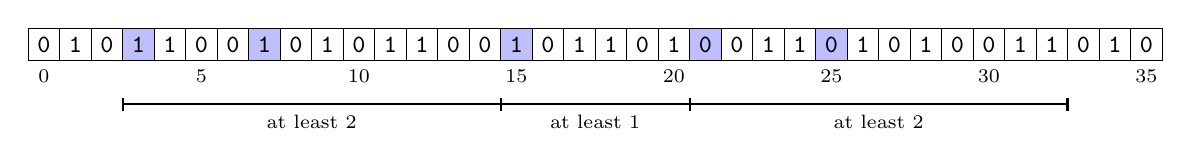
\begin{tikzpicture}[x=0.40cm,y=0.40cm]
\def\word{0,1,0,1,1,0,0,1,0,1,0,1,1,0,0,1,0,1,1,0,1,0,0,1,1,0,1,0,1,0,0,1,1,0,1,0}
\foreach \p in {3,7,15,21,25} {\fill[blue!25] (\p,0) rectangle +(1,1);}
\foreach \c [count=\i from 0] in \word {
  \draw (\i,0) rectangle +(1,1);
  \node at (\i+0.5,0.5) {\small\texttt{\c}};
}
\foreach \i in {0,5,10,15,20,25,30,35} {\node[below] at (\i+0.5,0) {\scriptsize\i};}
\draw[thick] (3,-1.4) -- (15,-1.4) node[midway,below] {\scriptsize at least $2$};
\draw[thick] (15,-1.4) -- (21,-1.4) node[midway,below] {\scriptsize at least $1$};
\draw[thick] (21,-1.4) -- (33,-1.4) node[midway,below] {\scriptsize at least $2$};
\foreach \x in {3,15,21,33} {\draw[thick] (\x,-1.2) -- (\x,-1.6);}
\end{tikzpicture}
\caption{The prefix $w_5$, positions $0$ to $35$, with the attractor
$\Gamma=\{3,7,15,21,25\}$ shaded. Below it are the three disjoint regions
$[3,14]$, $[15,20]$ and $[21,32]$ of the lower-bound proof, with the number
of positions each must contain.}
\label{fig:word}
\end{figure}

\subsection*{What is new, and the hard step}
Dvořáková and Hendrychová's conjecture rests on their computer experiments.
The subclass results---Dvořáková's standard Sturmian
result~\cite{d-epi}, restated and re-proved in~\cite{dh}, and the
pseudostandard and standard complementary-symmetric Rote results of
Dvořáková and Hendrychová~\cite{dh}---are untouched by Theorem~\ref{thm:main}. The word $w_5$ has ten distinct factors of length four,
while a Sturmian sequence has five and a Rote sequence eight~\cite{rote}, so
$w_5$ is a factor of neither; and $w_5$ is a palindrome, not one of the
antipalindromic prefixes that \cite[Theorem~8]{dh} describes. What this note
adds is a prefix outside these classes that needs five positions. The upper bound is a
direct check. The hard step is the lower bound: that no four positions form an
attractor. A priori this means ruling out every set of four positions; we
replace that by seven factors whose occurrences force five positions
(Section~\ref{sec:lower}).

\subsection*{Proof overview and map}
Section~\ref{sec:defs} quotes the definitions and the conjecture.
Section~\ref{sec:member} computes the five closures that produce $w_5$, so
that $w_5$ is a pseudopalindromic prefix exactly in the sense of the
conjecture. Section~\ref{sec:lower} proves the lower bound: an attractor must
meet the union of the occurrences of each factor, and seven factors, with
only one or two occurrences each, force at least two positions in $[3,14]$,
one in $[15,20]$ and two in $[21,32]$. Section~\ref{sec:upper} proves that
$\Gamma$ is an attractor, by reducing the check to the factors that occur inside a
gap of $\Gamma$, the end gaps included (listed in Appendix~\ref{app:table}). Section~\ref{sec:second} gives a second example,
of length $43$, and Section~\ref{sec:open} says what remains open.
Appendix~\ref{app:computer} describes the computer checks. The proof of
Theorem~\ref{thm:main} is complete without them; the second example rests on
them.

\section{Definitions and the conjecture}\label{sec:defs}

This section quotes the definitions of~\cite{dh} (arXiv version~5, which is
the published version) word for word, so that the example can be checked
against them. Section~2 of~\cite{dh} defines attractors: ``A string attractor
(or attractor for short) of a word $w=w_0w_1\cdots w_{n-1}$, where
$w_i\in\mathcal A$, is a set $\Gamma\subset\{0,1,\dots,n-1\}$ such that every
non-empty factor of $w$ has an occurrence in $w$ containing at least one
element of $\Gamma$.'' Here an occurrence of a factor
$w_iw_{i+1}\cdots w_{j-1}$ is the set of positions $\{i,i+1,\dots,j-1\}$.
Section~3 of~\cite{dh} defines, after its Definition~1 of $R$
and $E$:

\begin{quote}
``Consider $w\in\{0,1\}^*$. Then $w^R$ is the shortest palindrome having $w$
as prefix and it is called the palindromic closure of $w$. Similarly, $w^E$
is the shortest antipalindrome having $w$ as prefix and it is called the
antipalindromic closure of $w$.''

``Let $w\in\{0,1\}^+$. It follows immediately from the definition that
$w^R=vxR(v)$, where $w=vx$ and $x$ is the longest palindromic suffix of $w$.
Similarly, $w^E=vyE(v)$, where $y$ is the longest antipalindromic suffix of
$w$ (possibly empty).''
\end{quote}

\noindent Definition~3 of~\cite{dh} reads:
\begin{quote}
``\textbf{Definition 3.} Let $\Delta=\delta_1\delta_2\cdots$ and $\Theta=\vartheta_1\vartheta_2\cdots$,
where $\delta_i\in\{0,1\}$ and $\vartheta_i\in\{E,R\}$ for all
$i\in\mathbb N$, $i\geq1$. The sequence $\mathbf u(\Delta,\Theta)$, called
generalized pseudostandard sequence, is the sequence having prefixes $w_n$
obtained from the recurrence relation
\[
w_{n+1}=(w_n\delta_{n+1})^{\vartheta_{n+1}},\qquad w_0=\varepsilon.
\]
The bi-sequence $(\Delta,\Theta)$ is called the directive bi-sequence of the
word $\mathbf u(\Delta,\Theta)$.''
\end{quote}

The conjecture is not numbered in~\cite{dh}. It is stated in the abstract and
in Section~7 (Open problems); we number it here for reference.

\begin{conjecture}[Dvořáková and Hendrychová~\cite{dh}]\label{conj}
Abstract: ``We conjecture that the pseudopalindromic prefixes of any binary
generalized pseudostandard sequence have a minimal string attractor of size
at most four.'' Section~7: ``Based on computer experiments, we conjecture
that the size of minimal string attractors of pseudopalindromic prefixes of
binary generalized pseudostandard sequences is of size at most four.''
\end{conjecture}

\noindent In~\cite{dh} a \emph{minimal} attractor is one of minimum size
(Section~2 there), so the conjecture says that every such prefix has an
attractor of at most four positions. Definition~3 places no condition on
$(\Delta,\Theta)$, and neither statement of the conjecture adds one.

\section{The prefix \texorpdfstring{$w_5$}{w5}}\label{sec:member}

This section shows that $w_5$ is the fifth word of the recurrence in
Definition~3. Write $\vartheta(v)$ for $R(v)$ or $E(v)$. By the remark quoted
above, if the seed $w_{n-1}\delta_n$ is written as $vx$ with $x$ its longest
$\vartheta_n$-fixed suffix, then $w_n=vx\,\vartheta_n(v)$. Table~\ref{tab:steps}
lists the five steps for $\Delta=00101\cdots$ and $\Theta=EEEER\cdots$. In
steps~1 and~3 no nonempty suffix of the seed is fixed by $E$ (a single letter
never is), so $x$ is empty and $w_n$ has twice the length of the seed.

\begin{table}[ht]
\centering\small
\begin{tabular}{@{}cccllll@{}}
\toprule
$n$ & $\delta_n$ & $\vartheta_n$ & seed $w_{n-1}\delta_n=vx$ & $x$ & $\vartheta_n(v)$ & $|w_n|$\\
\midrule
1 & 0 & $E$ & \w{0} & $\varepsilon$ & \w{1} & 2\\
2 & 0 & $E$ & \w{0|10} & \w{10} & \w{1} & 4\\
3 & 1 & $E$ & \w{01011} & $\varepsilon$ & \w{00101} & 10\\
4 & 0 & $E$ & \w{0101100|1010} & \w{1010} & \w{1100101} & 18\\
5 & 1 & $R$ & \w{01011001010110010|11} & \w{11} & \w{01001101010011010} & 36\\
\bottomrule
\end{tabular}
\caption{The closures producing $w_5$. A bar separates $v$ from $x$ in the
seed, and $|w_n|$ is the length of $w_n$.}
\label{tab:steps}
\end{table}

The words are
\[
w_1=\w{01},\quad w_2=\w{0101},\quad w_3=\w{0101100101},\quad
w_4=\w{010110010101100101},
\]
and $w_5$ is the word of Theorem~\ref{thm:main}; it equals its reversal.

\begin{lemma}\label{lem:member}
For every directive bi-sequence $(\Delta,\Theta)$ with $\Delta$ beginning
$00101$ and $\Theta$ beginning $EEEER$, the word $w_5$ of Definition~3 is a
pseudopalindromic prefix of the generalized pseudostandard sequence
$\mathbf u(\Delta,\Theta)$.
\end{lemma}

\begin{proof}
The words $w_1,\dots,w_5$ depend only on the first five letters of $\Delta$
and $\Theta$, and Table~\ref{tab:steps} computes them. Each $w_{n+1}$ has the
word $w_n\delta_{n+1}$, one letter longer than $w_n$, as a prefix, so the $w_n$ are prefixes of one
another with strictly increasing lengths, and $\mathbf u(\Delta,\Theta)$ is the
infinite sequence they define. Thus $w_5$ is a prefix of it, and a palindrome.
\end{proof}

\noindent Counted by length, $w_5$ is the seventh nonempty pseudopalindromic
prefix of $\mathbf u(\Delta,\Theta)$: the prefixes of lengths $1,2,3,4,10,18$
and $36$ are fixed by $R$ or $E$. The conjecture covers it under either
reading, as a word $w_n$ of Definition~3 or as a pseudopalindromic prefix.

\begin{remark}
The conjecture asks for no further property of $\mathbf u(\Delta,\Theta)$, but
the example also lives in an aperiodic sequence. Take $\Delta=00101(01)^\omega$
and $\Theta=EEEER\,R^\omega$. Florian and Dvořáková~\cite{df} showed (see~\cite[Theorem~16]{dh}) that $\mathbf u(\Delta,\Theta)$ is eventually periodic exactly when some
bijection $f\colon\{E,R\}\to\{0,1\}$ satisfies $f(\vartheta_n)=\delta_{n+1}$ for
all large $n$. Here $\vartheta_n=R$ for $n\geq5$ while $\delta_{n+1}$ alternates,
so no such $f$ exists.
\end{remark}

\section{No four positions suffice}\label{sec:lower}

This section proves the lower bound of Theorem~\ref{thm:main}, the step that
refutes the conjecture. For a factor $f$ of $w_5$, let $C(f)$ be the set of
positions lying in at least one occurrence of $f$. A set $\Gamma$ attracts $f$
exactly when it meets $C(f)$. In blocks of six, starting at positions
$0,6,12,18,24,30$,
\[
w_5=\w{010110}\ \w{010101}\ \w{100101}\ \w{101001}\ \w{101010}\ \w{011010}.
\]

\begin{lemma}\label{lem:seven}
The following seven factors of $w_5$ occur exactly at the listed starting
positions, so their position sets are as shown.
\begin{center}\small\upshape
\begin{tabular}{@{}llll@{}}
\toprule
region & factor $f$ & starts & $C(f)$\\
\midrule
left   & $f_1=\w{001010}$ & 5 & $[5,10]$\\
left   & $f_2=\w{101011}$ & 7 & $[7,12]$\\
left   & $f_3=\w{1100}$ & 3, 11 & $[3,6]\cup[11,14]$\\
middle & $f_4=\w{101101}$ & 15 & $[15,20]$\\
right  & $f_5=\w{010100}$ & 25 & $[25,30]$\\
right  & $f_6=\w{110101}$ & 23 & $[23,28]$\\
right  & $f_7=\w{0011}$ & 21, 29 & $[21,24]\cup[29,32]$\\
\bottomrule
\end{tabular}
\end{center}
\end{lemma}

\begin{proof}
Each is found by reading $w_5$ in the display above. For instance $\w{1100}$
needs two consecutive ones followed by two zeros; the only $\w{11}$'s start at
$3,11,17,23,31,$ and only those at $3$ and $11$ are followed by $\w{00}$.
\end{proof}

\begin{proposition}\label{prop:lower}
Every string attractor of $w_5$ has at least five positions.
\end{proposition}

\begin{proof}
Let $\Gamma$ be an attractor; it meets each of the seven sets of
Lemma~\ref{lem:seven}. The three left sets lie in $[3,14]$. Their common
intersection is empty, since $C(f_1)\cap C(f_2)=[7,10]$ is disjoint from
$C(f_3)$. So no single position meets all three, and $\Gamma$ has at least two
positions in $[3,14]$. Likewise the right sets lie in $[21,32]$, and
$C(f_5)\cap C(f_6)=[25,28]$ is disjoint from $C(f_7)$, so $\Gamma$ has at least
two positions in $[21,32]$. Finally $\Gamma$ meets $C(f_4)=[15,20]$. The three
intervals $[3,14]$, $[15,20]$ and $[21,32]$ are disjoint, so
$|\Gamma|\geq2+1+2=5$.
\end{proof}

Faro, Marino and Pavone~\cite{faro} use the same kind of certificate, a few
factors whose occurrence sets force the size of every attractor, for the
Thue--Morse words. The proposition is also confirmed by computer
(Appendix~\ref{app:computer}): no set of four positions is an attractor, and
any set of fewer positions would be contained in one.

\section{Five positions suffice}\label{sec:upper}

This section proves that $\Gamma=\{3,7,15,21,25\}$ is an attractor of $w_5$,
which gives the upper bound. The positions of $\Gamma$ split the rest of the
word into the \emph{gaps} $[0,2]$, $[4,6]$, $[8,14]$, $[16,20]$, $[22,24]$ and
$[26,35]$.

\begin{lemma}\label{lem:gaps}
A set $\Gamma$ of positions of a word is an attractor if and only if every
factor of every gap word (the factor occupying a gap) has an occurrence that
contains a position of $\Gamma$.
\end{lemma}

\begin{proof}
An occurrence that contains no position of $\Gamma$ lies inside one gap. So a
factor all of whose occurrences miss $\Gamma$ is a factor of a gap word. The
converse is the definition.
\end{proof}

\begin{proposition}\label{prop:upper}
The set $\Gamma=\{3,7,15,21,25\}$ is a string attractor of $w_5$.
\end{proposition}

\begin{proof}
The six gap words are $\w{010}$, $\w{100}$, $\w{0101100}$, $\w{01101}$,
$\w{011}$ and $\w{1010011010}$. Together they have $48$ distinct factors.
Table~\ref{tab:gaps} in Appendix~\ref{app:table} gives, for each, a starting
position of an occurrence and a position of $\Gamma$ that this occurrence
contains. Lemma~\ref{lem:gaps} completes the proof.
\end{proof}

For example, the longest gap word $\w{1010011010}$ occupies $[26,35]$ and also
occurs at $[18,27]$, which contains $21$ and $25$.

\section{A second example}\label{sec:second}

This section records a second prefix that needs five positions; its lower
bound is checked only by computer. Take $\Delta$ beginning $001001$ and
$\Theta$ beginning $RRREER$. Table~\ref{tab:second} lists the six closures,
in the notation of Table~\ref{tab:steps}. They give $w_1=\w{0}$, $w_2=\w{00}$,
$w_3=\w{00100}$, then words of lengths $12$ and $24$, and finally the
palindrome of length $43$
\[
w_6=\w{0010001110110010001110111000100110111000100}.
\]

\begin{table}[ht]
\centering\small
\begin{tabular}{@{}cccllll@{}}
\toprule
$n$ & $\delta_n$ & $\vartheta_n$ & seed $w_{n-1}\delta_n=vx$ & $x$ & $\vartheta_n(v)$ & $|w_n|$\\
\midrule
1 & 0 & $R$ & \w{|0} & \w{0} & $\varepsilon$ & 1\\
2 & 0 & $R$ & \w{|00} & \w{00} & $\varepsilon$ & 2\\
3 & 1 & $R$ & \w{00|1} & \w{1} & \w{00} & 5\\
4 & 0 & $E$ & \w{001000} & $\varepsilon$ & \w{111011} & 12\\
5 & 0 & $E$ & \w{00100011101|10} & \w{10} & \w{01000111011} & 24\\
6 & 1 & $R$ & \w{001000111011001000|1110111} & \w{1110111} & \w{000100110111000100} & 43\\
\bottomrule
\end{tabular}
\caption{The closures producing $w_6$. A bar separates $v$ from $x$ in the seed.}
\label{tab:second}
\end{table}

\begin{proposition}\label{prop:second}
The smallest string attractor of $w_6$ has size five; $\{3,11,20,25,30\}$ is
one.
\end{proposition}

\noindent The proof is by computer (Appendix~\ref{app:computer}). We know no
short argument like Lemma~\ref{lem:seven} for $w_6$.

\section{What remains open}\label{sec:open}

Dvořáková and Hendrychová based the conjecture on computer experiments, and
the bound four is attained by the Thue--Morse sequence~\cite{kutsukake};
Theorem~\ref{thm:main} shows that it is exceeded already at length $36$.
The standard Sturmian result of Dvořáková~\cite{d-epi}, restated and
re-proved in~\cite{dh}, and the pseudostandard and standard
complementary-symmetric Rote results of Dvořáková and
Hendrychová~\cite{dh} are untouched, since
Theorem~\ref{thm:main} concerns a directive bi-sequence outside those
classes. We do not claim that $w_5$ is the shortest counterexample. Whether
some constant bounds the attractor sizes of all these prefixes, and if so the
best constant, remains open.

\begin{appendices}

\section{The 48 factors of the gap words}\label{app:table}

Table~\ref{tab:gaps} lists every distinct factor of the six gap words of
Section~\ref{sec:upper}, by length, with the start $s$ of an occurrence in
$w_5$ and a position $p\in\Gamma$ with $s\leq p\leq s+|f|-1$. The same table
is the file \file{data/upper-bound.json} in the result's folder.

\begin{table}[ht]
\centering\small
\begin{tabular}{@{}lrr@{\qquad}lrr@{\qquad}lrr@{}}
\toprule
factor & $s$ & $p$ & factor & $s$ & $p$ & factor & $s$ & $p$\\
\midrule
\texttt{0} & 21 & 21 & \texttt{1001} & 4 & 7 & \texttt{010110} & 0 & 3 \\
\texttt{1} & 3 & 3 & \texttt{1010} & 7 & 7 & \texttt{011010} & 16 & 21 \\
\texttt{00} & 21 & 21 & \texttt{1011} & 1 & 3 & \texttt{100110} & 20 & 21 \\
\texttt{01} & 2 & 3 & \texttt{1100} & 3 & 3 & \texttt{101001} & 18 & 21 \\
\texttt{10} & 7 & 7 & \texttt{1101} & 23 & 25 & \texttt{101100} & 1 & 3 \\
\texttt{11} & 3 & 3 & \texttt{00110} & 21 & 21 & \texttt{0011010} & 21 & 21 \\
\texttt{001} & 5 & 7 & \texttt{01001} & 19 & 21 & \texttt{0100110} & 19 & 21 \\
\texttt{010} & 6 & 7 & \texttt{01011} & 0 & 3 & \texttt{0101100} & 0 & 3 \\
\texttt{011} & 2 & 3 & \texttt{01100} & 2 & 3 & \texttt{1001101} & 20 & 21 \\
\texttt{100} & 20 & 21 & \texttt{01101} & 22 & 25 & \texttt{1010011} & 18 & 21 \\
\texttt{101} & 1 & 3 & \texttt{10011} & 20 & 21 & \texttt{01001101} & 19 & 21 \\
\texttt{110} & 3 & 3 & \texttt{10100} & 18 & 21 & \texttt{10011010} & 20 & 21 \\
\texttt{0011} & 21 & 21 & \texttt{10110} & 1 & 3 & \texttt{10100110} & 18 & 21 \\
\texttt{0100} & 19 & 21 & \texttt{11010} & 17 & 21 & \texttt{010011010} & 19 & 21 \\
\texttt{0101} & 0 & 3 & \texttt{001101} & 21 & 21 & \texttt{101001101} & 18 & 21 \\
\texttt{0110} & 2 & 3 & \texttt{010011} & 19 & 21 & \texttt{1010011010} & 18 & 21 \\
\bottomrule
\end{tabular}
\caption{Each factor of a gap word, with an occurrence starting at $s$ that
contains the position $p$ of $\Gamma$.}
\label{tab:gaps}
\end{table}

\section{Computer checks}\label{app:computer}

Two programs, written independently and using only the Python standard
library, check the claims from the definitions. They are in the folder that
accompanies this paper, whose \file{checks/README.md} explains how to run
them.

The first, \file{checks/check_exhaustive.py}, rebuilds each closure as the
shortest word fixed by $R$ or $E$ with the given prefix, trying the lengths in
increasing order. It checks that the listed five positions attract every
factor, and tests every set of four positions: none of the
$\binom{36}{4}=58{,}905$ sets for $w_5$ and none of the
$\binom{43}{4}=123{,}410$ sets for $w_6$ is an attractor. Adding positions to
an attractor gives an attractor, and a word of length at least four has a
set of four positions containing any smaller set, so sets of fewer than four
positions are excluded too. As controls it reproduces Example~2 and
Example~4 of~\cite{dh} and the attractor $\{1,3\}$ of $\w{010010}$.

The second, \file{checks/check_proof.py}, rebuilds each closure by the
longest-suffix formula and confirms by trying every shorter extension that
no shorter fixed word exists. It checks Lemma~\ref{lem:seven} and the
proof of Proposition~\ref{prop:lower} (complete occurrence lists, empty
intersections, disjoint regions), checks Table~\ref{tab:gaps} against the
gaps of $\Gamma$, and computes the smallest attractor size of $w_5$ and $w_6$
by a branch-and-bound search for a smallest set of positions meeting every
$C(f)$. Both programs reject corrupted inputs: a flipped letter, a changed
closure type, five positions that are not an attractor, a Thue--Morse prefix
(which has an attractor of size four), and, for the second program, a missing
occurrence or factor in the obstruction or the table. The whole check takes a
few seconds.

\end{appendices}

\begin{thebibliography}{9}

\bibitem{banbara}
M.~Banbara, H.~Bannai, P.~Guo, D.~Köppl, T.~Mieno and Y.~Okamoto,
\emph{The smallest string attractors of Fibonacci, period-doubling, and
Thue--Morse words}, \href{https://arxiv.org/abs/2602.16152}{arXiv:2602.16152}, 2026.

\bibitem{bptv}
A.~Blondin Massé, G.~Paquin, H.~Tremblay and L.~Vuillon,
\emph{On generalized pseudostandard words over binary alphabets},
J.\ Integer Seq.\ \textbf{16} (2013), Article 13.2.11.

\bibitem{dldl}
A.~de~Luca and A.~De~Luca,
\emph{Pseudopalindrome closure operators in free monoids},
Theoret.\ Comput.\ Sci.\ \textbf{362} (2006), 282--300.

\bibitem{d-epi}
L.~Dvořáková,
\emph{String attractors of episturmian sequences},
Theoret.\ Comput.\ Sci.\ \textbf{986} (2024), 114341.

\bibitem{dh}
L.~Dvořáková and V.~Hendrychová,
\emph{String attractors of Rote sequences},
Discrete Math.\ Theor.\ Comput.\ Sci.\ \textbf{26}:3 (2024), \#2,
\href{https://doi.org/10.46298/dmtcs.12385}{doi:10.46298/dmtcs.12385},
\href{https://arxiv.org/abs/2308.00850}{arXiv:2308.00850}, first posted August 1, 2023.

\bibitem{faro}
S.~Faro, F.~P.~Marino and A.~Pavone,
\emph{Smallest string attractors and minimal coverage certificates of
Thue--Morse words}, \href{https://arxiv.org/abs/2610.10950}{arXiv:2610.10950}, 2026.

\bibitem{df}
J.~Florian and L.~Dvořáková,
\emph{On periodicity of generalized pseudostandard words},
Electron.\ J.\ Combin.\ \textbf{23} (2016), P1.2.

\bibitem{kp}
D.~Kempa and N.~Prezza,
\emph{At the roots of dictionary compression: string attractors},
in Proc.\ 50th ACM Symposium on Theory of Computing (STOC 2018), 827--840.

\bibitem{kutsukake}
K.~Kutsukake, T.~Matsumoto, Y.~Nakashima, S.~Inenaga, H.~Bannai and M.~Takeda,
\emph{On repetitiveness measures of Thue--Morse words},
in String Processing and Information Retrieval (SPIRE 2020),
Lecture Notes in Comput.\ Sci.\ \textbf{12303}, Springer, 2020, 213--220.

\bibitem{rote}
G.~Rote,
\emph{Sequences with subword complexity $2n$},
J.\ Number Theory \textbf{46} (1994), 196--213.

\end{thebibliography}
\end{document}
